\documentclass[conference]{IEEEtran}
\IEEEoverridecommandlockouts
% The preceding line is only needed to identify funding in the first footnote. If that is unneeded, please comment it out.
\usepackage{cite}
\usepackage{amsmath,amssymb,amsfonts}
\usepackage{algorithmic}
\usepackage{graphicx}
\usepackage{textcomp}
\usepackage{xcolor}
\usepackage[brazilian]{babel}
\usepackage[utf8]{inputenc}
\usepackage[T1]{fontenc}
\usepackage{listings}
\usepackage{listings-golang}
\usepackage{color}
\usepackage{float}
\usepackage{multirow}
\usepackage{hyperref}

\definecolor{dkgreen}{rgb}{0,0.6,0}
\definecolor{gray}{rgb}{0.5,0.5,0.5}
\definecolor{mauve}{rgb}{0.58,0,0.82}

\lstset{frame=tb,
  language=Golang,
  aboveskip=3mm,
  belowskip=3mm,
  showstringspaces=false,
  columns=flexible,
  basicstyle={\small\ttfamily},
  numbers=none,
  numberstyle=\tiny\color{gray},
  keywordstyle=\color{blue},
  commentstyle=\color{dkgreen},
  stringstyle=\color{mauve},
  breaklines=true,
  breakatwhitespace=true,
  tabsize=3
}
\lstset{language=Golang}
\def\BibTeX{{\rm B\kern-.05em{\sc i\kern-.025em b}\kern-.08em
    T\kern-.1667em\lower.7ex\hbox{E}\kern-.125emX}}
\begin{document}

\title{Relatório da Atividade 3: \\ Map Reduce\\
}

\author{\IEEEauthorblockN{Isabelle Ferreira de Oliveira}
\IEEEauthorblockA{\textit{CES-27 - Engenharia da Computação 2020} \\
\textit{Instituto Tecnológico de Aeronáutica (ITA)}\\
São José dos Campos, Brasil \\
isabelle.ferreira3000@gmail.com}
}

\maketitle

\begin{abstract}
Esse relatório documenta um trabalho com o modelo de programação MapReduce de forma sequencial e distribuída.
\end{abstract}

\begin{IEEEkeywords}
Map Reduce, Golang, sistema sequencial, sistema distribuído
\end{IEEEkeywords}

\section{Implementação}

\subsection{Parte 1: Trabalhando em modo sequencial}

\subsubsection{Tarefa 1.1} Bastou percorrer a lista de palavras presentes em \textit{words} e, para cada palavra, adicionar a um array de mapreduce.KeyValue um novo item, contendo a palavra em questão como atributo \textit{Key} e "1" como atributo \textit{Value}.

\begin{lstlisting}
func mapFunc(input []byte) (result []mapreduce.KeyValue) {

	// [...]

	var item mapreduce.KeyValue

	for _, word := range words {
		word = strings.ToLower(word)
		item.Key = word
		item.Value = "1"
		result = append(result, item)
	}
	
	return result
}
\end{lstlisting}

\subsubsection{Tarefa 1.2} Bastou percorrer o array \textit{input} de mapreduce.KeyValue, atualizando um mapa a fim de agrupar as palavras repetidas nesse \textit{input}. O atributo Key de cada item desse \textit{input} era a palavra que serviria de chave nesse mapa. Caso a palavra já estivesse no mapa, acrescentava-se o valor contido no atributo Value do item ao valor já presente no mapa. Caso contrário, esse novo item era adicionado no mapa, com o atributo Value sendo setado como valor inicial dessa chave. Após isso, percorreu-se esse mapa, adicionando os elementos no array \textit{result} de mapreduce.KeyValue. Era necessário, também, vazer as conversões de inteiro para string, e vice-versa, para adicionar corretamente nos mapas e no array \textit{result} de mapreduce.KeyValue.

\begin{lstlisting}
func reduceFunc(input []mapreduce.KeyValue) (result []mapreduce.KeyValue) {

	var mapAux map[string]int = make(map[string]int)
	var value int

	for _,item := range input {
		value, _ = strconv.Atoi(item.Value)
		_, ok := mapAux[item.Key]
		if ok {
			mapAux[item.Key] += value
		} else {
			mapAux[item.Key] = value
		}
	}

	var itemAux mapreduce.KeyValue

	for key,value := range mapAux {
		itemAux.Key = key
		itemAux.Value = strconv.Itoa(value)
		result = append(result, itemAux)
	}
	
	return result
}
\end{lstlisting}

\subsubsection{Tarefa 1.3} Executou-se o comando \textit{"./wordcount -mode sequential -file files/teste.txt -chunksize 100 -reducejobs 2"}, conforme sugerido no roteiro.

\subsubsection{Tarefa 1.4} Executou-se o comando da Tarefa 1.3, dessa vez para o arquivo \textit{files/musica.txt}. Os valores de \textit{chunksize} e \textit{reducejob} foram alterados para: 100 e 2; 100 e 1; e 102400 e 2. O arquivo \textit{musica.txt} pode ser observado no código enviado em anexo ao relatório.

\subsection{Parte 2: Trabalhando em modo distribuído}

\subsubsection{Tarefa 2.1} Blabla

\begin{lstlisting}
func (master *Master) handleFailingWorkers() {

	for elem := range master.failedWorkerChan {
		master.workersMutex.Lock()
		delete(master.workers, elem.id)
		master.totalWorkers--
		master.workersMutex.Unlock()

		fmt.Println("Removing worker", elem.id, "from master list")
	}
}
\end{lstlisting}

\subsubsection{Tarefa 2.2} Blabla

\begin{lstlisting}
type Master struct {
	// [...]

	// Fault Tolerance
	failedOperationChan chan *Operation
}
\end{lstlisting}

\begin{lstlisting}
func (master *Master) runOperation(remoteWorker *RemoteWorker, operation *Operation, wg *sync.WaitGroup) {

	// [...]

	if err != nil {
		log.Printf("Operation %v '%v' Failed. Error: %v\n", operation.proc, operation.id, err)
		
		master.failedWorkerChan <- remoteWorker
		master.failedOperationChan <- operation
	} else {
		wg.Done()
		master.idleWorkerChan <- remoteWorker
	}
}
\end{lstlisting}

\begin{lstlisting}
func (master *Master) handleFailingOperations(wg *sync.WaitGroup) {

	var operation *Operation
	var worker *RemoteWorker
	var ok bool

	for {
		operation, ok = <-master.failedOperationChan
		if !ok { break }

		worker, _ = <-master.idleWorkerChan

		go master.runOperation(worker, operation, wg)
	}
}
\end{lstlisting}

\begin{lstlisting}
func (master *Master) schedule(task *Task, proc string, filePathChan chan string) int {

	var (
		wg        sync.WaitGroup
		filePath  string
		worker    *RemoteWorker
		operation *Operation
		counter   int
	)
	
	master.failedOperationChan = make(chan *Operation, RETRY_OPERATION_BUFFER)

	go master.handleFailingOperations(&wg)

	// [...]
}
\end{lstlisting}

\subsubsection{Tarefa 2.3}

\subsubsection{Tarefa 2.4}


\section{Resultados e Conclusões} \label{results}

\subsection{Teste 1}

	Este foi o caso com um processo solicitando a CS e, depois que ele liberasse, outro processo solicitando a CS, sugerido no roteiro do laboratório. O esquema do resultado esperado foi apresentado na Figura \ref{ex1}.
	
	Na Figura \ref{ex1}, para P1, as setas azuis representam requests e as verdes, replies; para P3, essa setas são rosas e cinzas, respectivamente. Nos requests, a mensagem enviada é da forma "\textit{relógio lógico, < timestamp, id >}"; já no reply, a forma é "\textit{relógio lógico, 'reply'}". Além disso, a linha amarela representa o processo no estado WANTED; e a linha vermelha, no estado HELD, ou seja, na CS.
	
\begin{figure}[H]
\centering
\centerline{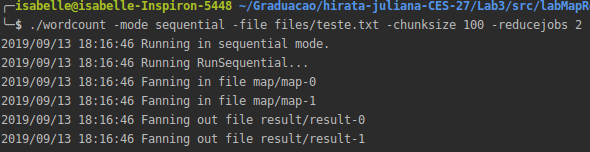
\includegraphics[scale=0.3]{imagens/tarefa_1_3/tarefa_1_3.png}}
\caption{Teste}
\label{ex1}
\end{figure}

	Foi simulada essa situação acima com o código implementado no laboratório, tendo os resultados apresentados nas Figuras de \ref{ex1-proc1-clean} a \ref{ex1-shared-clean}. Na simulação, ao invés de o P3 fazer a requisição, é o P2 a faz, mas isso não prejudica o teste.
	
\begin{figure}[H]
\centering
\centerline{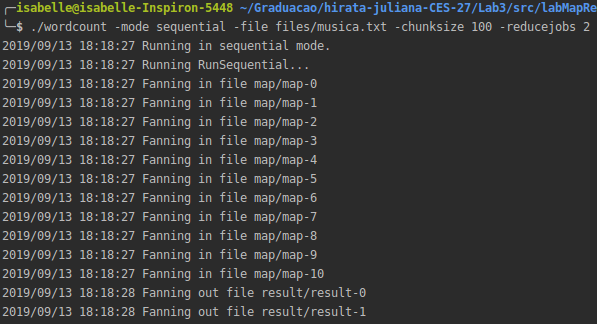
\includegraphics[scale=0.5]{imagens/tarefa_1_4_1/tarefa_1_4_1.png}}
\caption{Exemplo do funcionamento da tarefa com 3 processos. Tela do processo 1.}.
\label{ex1-proc1-clean}
\end{figure}

\begin{figure}[H]
\centering
\centerline{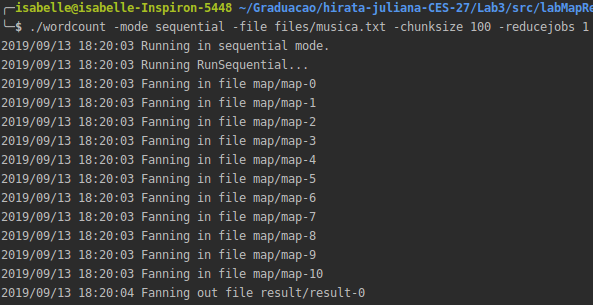
\includegraphics[scale=0.5]{imagens/tarefa_1_4_2/tarefa_1_4_2.png}}
\caption{Exemplo do funcionamento da tarefa com 3 processos. Tela do processo 2.}.
\label{ex1-proc2-clean}
\end{figure}

\begin{figure}[H]
\centering
\centerline{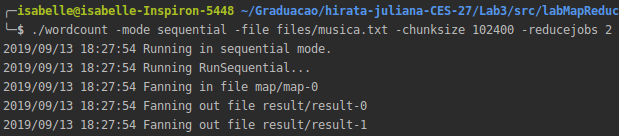
\includegraphics[scale=0.5]{imagens/tarefa_1_4_3/tarefa_1_4_3.png}}
\caption{Exemplo do funcionamento da tarefa com 3 processos. Tela do processo 3.}.
\label{ex1-proc3-clean}
\end{figure}

\begin{figure}[H]
\centering
\centerline{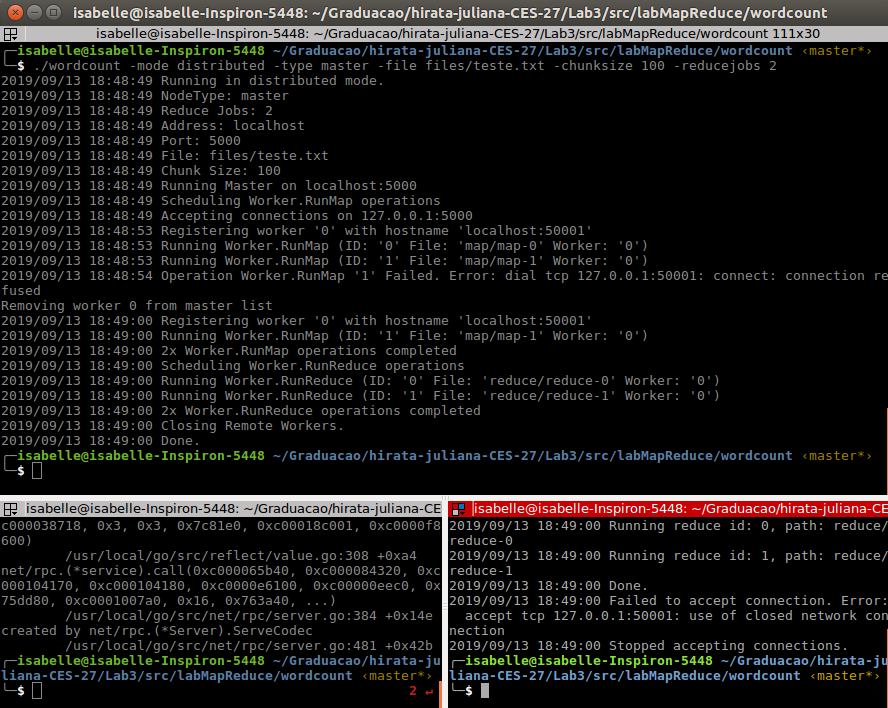
\includegraphics[scale=0.5]{imagens/tarefa_2_3_map/tarefa_2_3_map.png}}
\caption{Exemplo do funcionamento da tarefa com 3 processos. Tela do SharedResource.}.
\label{ex1-shared-clean}
\end{figure}
	
	A fim de entender melhor cada estágio do funcionamento, foram realizados os mesmos testes novamente, agora com prints de debug. Dessa forma, esses resultados estão apresentados nas Figuras de \ref{ex1-proc1} a \ref{ex1-shared}.
	
\begin{figure}[H]
\centering
\centerline{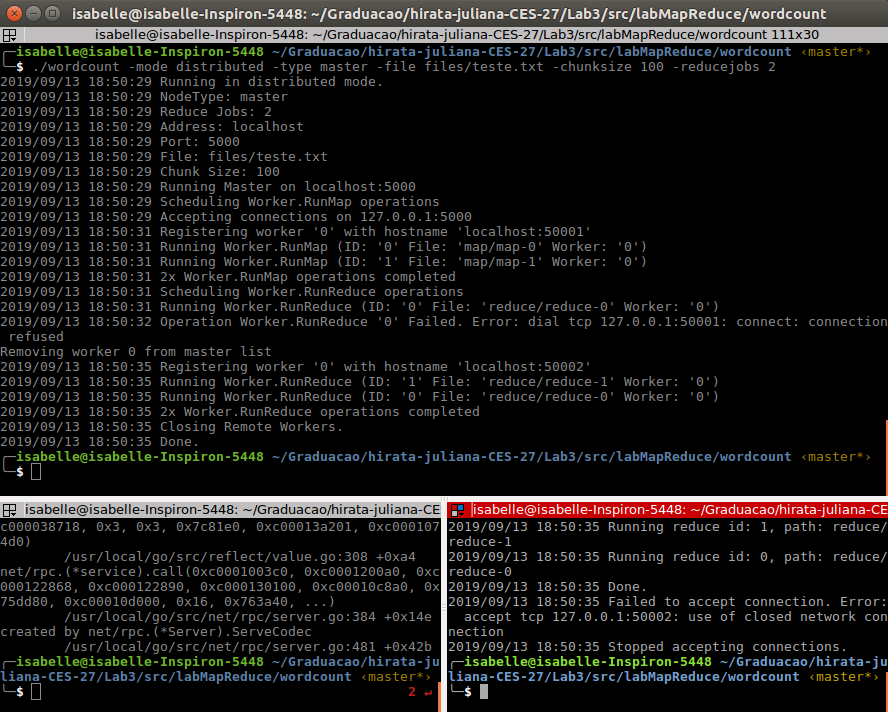
\includegraphics[scale=0.5]{imagens/tarefa_2_3_reduce/tarefa_2_3_reduce.png}}
\caption{Exemplo do funcionamento da tarefa com 3 processos. Tela do processo 1.}.
\label{ex1-proc1}
\end{figure}

\begin{figure}[H]
\centering
\centerline{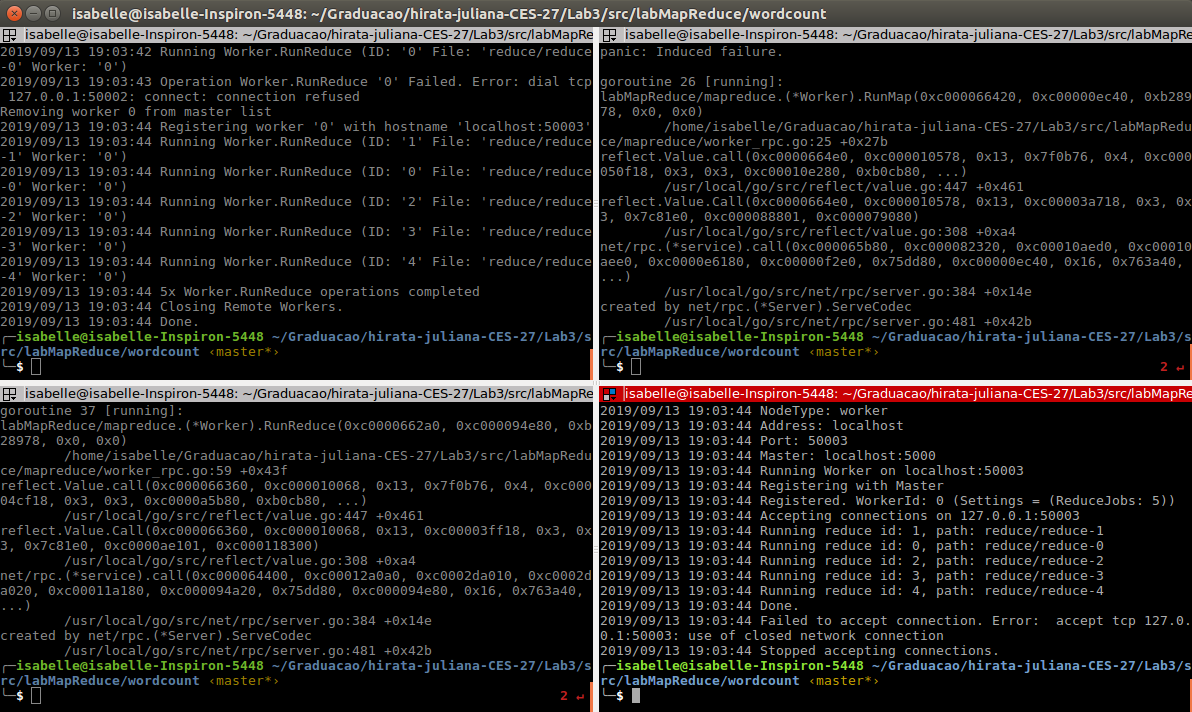
\includegraphics[scale=0.5]{imagens/tarefa_2_4_1/tarefa_2_4_1.png}}
\caption{Exemplo do funcionamento da tarefa com 3 processos. Tela do processo 2.}.
\label{ex1-proc2}
\end{figure}

\begin{figure}[H]
\centering
\centerline{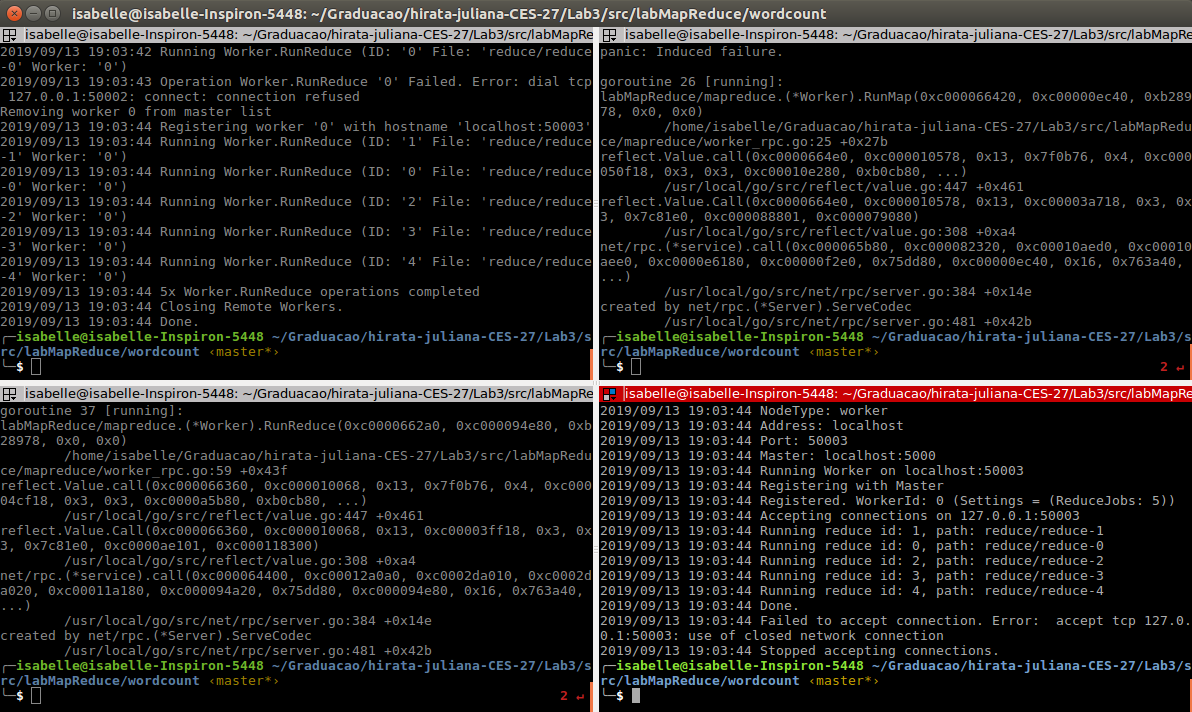
\includegraphics[scale=0.5]{imagens/tarefa_2_4_1/tarefa_2_4_1.png}}
\caption{Exemplo do funcionamento da tarefa com 3 processos. Tela do processo 3.}.
\label{ex1-proc3}
\end{figure}


	Como esses resultados foram condizentes com os resultados esperados, leva-se a perceber que a implementação da Tarefa foi feita corretamente. Mas, antes de concluir-se algo, foi-se realizado um segundo teste.

\subsection{Teste 2}

	Este foi o caso com processos solicitando a CS "simultaneamente", sugerido no roteiro do laboratório. O esquema do resultado esperado foi apresentado na Figura \ref{ex2}.
	
	Análogo ao teste 1, na Figura \ref{ex2}, para P1, as setas azuis representam requests e as verdes, replies; e para P4, essa setas são rosas e cinzas, respectivamente. Nos requests, a mensagem enviada também é da forma "\textit{relógio lógico, < timestamp, id >}"; assim como no reply, que a forma também é "\textit{relógio lógico, 'reply'}". Além disso, nesse caso também a linha amarela representa o processo no estado WANTED; e a linha vermelha, no estado HELD, ou seja, na CS.


	Foi simulada essa situação acima com o código implementado no laboratório, tendo os resultados apresentados nas Figuras de \ref{ex2-proc1-clean} a \ref{ex2-shared-clean}. Durante o período na CS, também foi digitado mensagens no terminal dos processos, para que se verifisse o funcionamento da validação da mensagem. Assim, para essas mensagens, foi dado o feedback de mensagem inválida.

	A fim de entender melhor cada estágio do funcionamento, foram realizados os mesmos testes novamente, agora com prints de debug. Dessa forma, esses resultados estão apresentados nas Figuras de \ref{ex2-proc1} a \ref{ex2-shared}. Como é difícil simular com exatidão os instantes dos envios de request dos processos simultaneamente, foi feito da seguinte forma: o processo P4 entra no estado WANTED durante o estado HELD do processo P1. Isso é um pouco diferente do apresentado na Figura \ref{ex2}, mas não prejudica os testes. Contudo, isso altera um pouco a ordem dos envios de mensagens, e, consequentemente, os valores relógios lógicos.


	
	Como esses resultados também foram condizentes com os resultados esperados, conclui-se que a implementação da Tarefa foi feita corretamente.
	
%\begin{thebibliography}{00}
%\bibitem{roteiro} M. Maximo, ``Roteiro: Laboratório 12 - Deep Q-Learning''. Instituto Tecnológico de Aeronáutica, Departamento de Computação. CT-213, 2019.

%\bibitem{roteiro8} M. Maximo, ``Roteiro: Laboratório 8 - Imitation Learning com Keras''. Instituto Tecnológico de Aeronáutica, Departamento de Computação. CT-213, 2019.

%\bibitem{roteiro12} M. Maximo, ``Roteiro: Laboratório 12 - Aprendizado por Reforço Livre de Modelo''. Instituto Tecnológico de Aeronáutica, Departamento de Computação. CT-213, 2019.

%\end{thebibliography}

\end{document}
